\documentclass[tikz,border=5pt]{standalone}
\usepackage{tikz}
\usepackage{amsmath}
\begin{document}

\begin{figure}[h]
\begin{center}
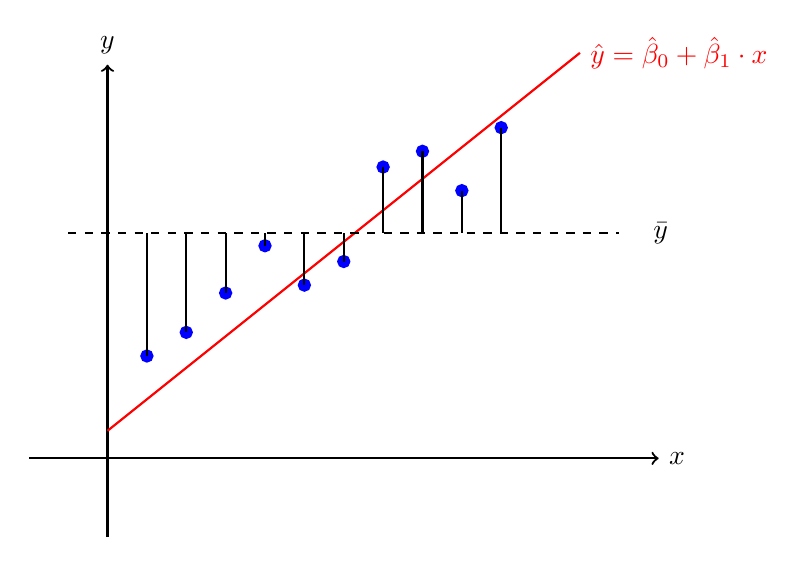
\begin{tikzpicture}[thick]
  \draw[->] (-1,0) -- (7,0) node[right] {$x$};
  \draw[->] (0,-1) -- (0,5) node[above] {$y$};
  \filldraw[blue] (0.5, 1.3) circle (2pt);
  \filldraw[blue] (1.5, 2.1) circle (2pt);
  \filldraw[blue] (1, 1.6) circle (2pt);
  \filldraw[blue] (2, 2.7) circle (2pt);
  \filldraw[blue] (2.5, 2.2) circle (2pt);
  \filldraw[blue] (3, 2.5) circle (2pt);
  \filldraw[blue] (3.5, 3.7) circle (2pt);
  \filldraw[blue] (4, 3.9) circle (2pt);
  \filldraw[blue] (4.5, 3.4) circle (2pt);
  \filldraw[blue] (5, 4.2) circle (2pt);
  \draw[red, thick, domain=0:6] plot (\x, {0.8*\x + 0.35}) node[right] {$\hat{y} = \hat{\beta}_0 + \hat{\beta}_1 \cdot x$};
  \draw[dashed] (-0.5,2.86) -- (6.5,2.86);
  \node at (6.8, 2.86) [right] {$\bar{y}$};
  \foreach \x/\y in {
    0.5/1.3,
    1.5/2.1,
    1/1.6,
    2/2.7,
    2.5/2.2,
    3/2.5,
    3.5/3.7,
    4/3.9,
    4.5/3.4,
    5/4.2
  } {
    \draw[black] (\x,\y) -- (\x,2.86);
  }
\end{tikzpicture}
\end{center}
\caption{An illustration of Total Sum of Squares (SST). The blue points represent height measurements over time, the dashed line is the mean height $\bar{y}$, and the solid black vertical lines represent the squared deviations from the mean (SST components).}
\end{figure}

\end{document}